\documentclass[tikz,border=10pt]{standalone}
\usepackage{amsmath,amssymb}
\usepackage{tikz}
\usetikzlibrary{arrows.meta,calc,positioning}

\definecolor{navy}{HTML}{1B365D}
\definecolor{steelblue}{HTML}{2471A3}
\definecolor{teal}{HTML}{0E6251}
\definecolor{amber}{HTML}{D35400}
\definecolor{crimson}{HTML}{C0392B}
\definecolor{slate}{HTML}{566573}

\begin{document}
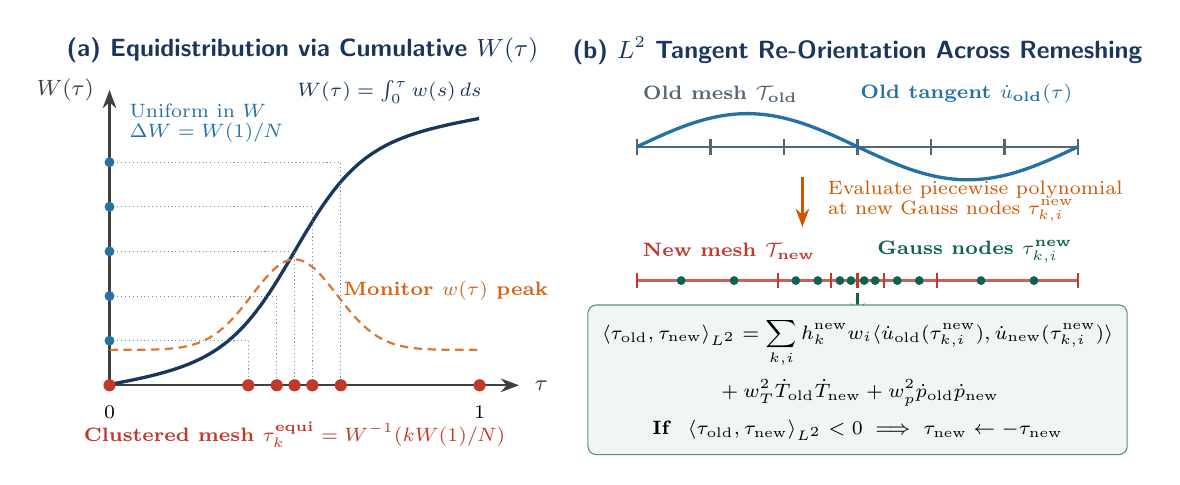
\begin{tikzpicture}[
    >=Stealth,
    font=\sffamily\small,
]

% ========================
% LEFT PANEL (a): Equidistribution via W^{-1}
% ========================
\begin{scope}[shift={(0,0)}]
    \node[font=\sffamily\bfseries\small, navy] at (2.80, 5.10)
        {(a) Equidistribution via Cumulative $W(\tau)$};

    % Axes
    \draw[->, thick, black!75] (0.35, 0.85) -- (5.55, 0.85) node[right=2pt, font=\footnotesize] {$\tau$};
    \draw[->, thick, black!75] (0.35, 0.85) -- (0.35, 4.60) node[left=2pt, font=\footnotesize] {$W(\tau)$};

    % Steep sigmoid W(tau) on x in [0.35, 5.05] (span 4.7)
    \draw[very thick, navy, domain=0:1, samples=100, smooth]
        plot ({0.35 + 4.7*\x}, {0.85 + 3.40*(0.22*\x + 0.78/(1 + exp(-11*(\x - 0.5))))});

    % Subtle background steep monitor w(tau) peak (dashed amber)
    \draw[thick, amber!80, densely dashed, domain=0:1, samples=100, smooth]
        plot ({0.35 + 4.7*\x}, {1.30 + 1.15*exp(-38*(\x - 0.5)*(\x - 0.5))});
    \node[amber!90, font=\scriptsize\bfseries, anchor=west] at (3.20, 2.05) {Monitor $w(\tau)$ peak};

    % Equal divisions on W-axis and inverse projection onto tau-axis
    \foreach \k/\tval in {1/0.375, 2/0.452, 3/0.500, 4/0.548, 5/0.625} {
        \pgfmathsetmacro{\yval}{0.85 + 3.40*\k/6.0}
        \pgfmathsetmacro{\xval}{0.35 + 4.7*\tval}
        \draw[thin, steelblue!75, densely dotted] (0.35, \yval) -- (\xval, \yval) -- (\xval, 0.85);
        \fill[steelblue] (0.35, \yval) circle (1.8pt);
        \fill[crimson] (\xval, 0.85) circle (2.2pt);
    }
    % Endpoints
    \fill[crimson] (0.35, 0.85) circle (2.2pt);
    \fill[crimson] (5.05, 0.85) circle (2.2pt);
    \node[below=3pt, font=\scriptsize] at (0.35, 0.82) {$0$};
    \node[below=3pt, font=\scriptsize] at (5.05, 0.82) {$1$};

    % Annotations
    \node[steelblue, font=\scriptsize, align=left, anchor=west] at (0.48, 4.18)
        {Uniform in $W$\\[-1pt]$\Delta W = W(1)/N$};
    \node[crimson, font=\scriptsize\bfseries, align=center] at (2.70, 0.22)
        {Clustered mesh $\tau_k^{\text{equi}} = W^{-1}(k W(1)/N)$};
    \node[navy, font=\scriptsize\bfseries, anchor=south east] at (5.20, 4.30) {$W(\tau) = \int_0^\tau w(s)\,ds$};
\end{scope}

% ========================
% RIGHT PANEL (b): Continuous L2 Tangent Transfer
% ========================
\begin{scope}[shift={(6.75, 0)}]
    \node[font=\sffamily\bfseries\small, navy] at (3.10, 5.10)
        {(b) $L^2$ Tangent Re-Orientation Across Remeshing};

    % Old mesh bar
    \node[slate, font=\scriptsize\bfseries, anchor=west] at (0.25, 4.55) {Old mesh $\mathcal{T}_{\text{old}}$};
    \node[steelblue, font=\scriptsize\bfseries, anchor=east] at (5.95, 4.55) {Old tangent $\dot{u}_{\text{old}}(\tau)$};
    \draw[thick, slate] (0.30, 3.88) -- (5.90, 3.88);
    \foreach \k in {0,...,6} {
        \pgfmathsetmacro{\xval}{0.30 + 5.60*\k/6.0}
        \draw[thick, slate] (\xval, 3.78) -- (\xval, 3.98);
    }
    % Old tangent curve along old mesh
    \draw[very thick, steelblue, domain=0:1, samples=80, smooth]
        plot ({0.30 + 5.60*\x}, {3.88 + 0.42*sin(360*\x)});

    % Interpolation arrow down to new Gauss points
    \draw[->, thick, amber] (2.40, 3.50) -- (2.40, 2.86);
    \node[font=\scriptsize, amber, align=left, anchor=west] at (2.60, 3.18)
        {Evaluate piecewise polynomial\\[-1pt]at new Gauss nodes $\tau_{k,i}^{\text{new}}$};

    % New mesh bar (clustered near center)
    \node[crimson, font=\scriptsize\bfseries, anchor=west] at (0.25, 2.55) {New mesh $\mathcal{T}_{\text{new}}$};
    \node[teal, font=\scriptsize\bfseries, anchor=east] at (5.95, 2.55) {Gauss nodes $\tau_{k,i}^{\text{new}}$};
    \draw[thick, crimson!80] (0.30, 2.18) -- (5.90, 2.18);
    \foreach \tval in {0.0, 0.32, 0.44, 0.50, 0.56, 0.68, 1.0} {
        \pgfmathsetmacro{\xval}{0.30 + 5.60*\tval}
        \draw[thick, crimson] (\xval, 2.08) -- (\xval, 2.28);
    }
    % Gauss dots inside clustered intervals
    \foreach \tval in {0.10, 0.22, 0.36, 0.41, 0.46, 0.485, 0.515, 0.54, 0.59, 0.64, 0.78, 0.90} {
        \pgfmathsetmacro{\xval}{0.30 + 5.60*\tval}
        \fill[teal] (\xval, 2.18) circle (1.6pt);
    }

    % Arrow into box
    \draw[->, thick, teal] (3.10, 2.02) -- (3.10, 1.66);

    % Compact two-line inner product sign-alignment box
    \node[draw=teal!70, fill=teal!6, rounded corners=3pt, font=\scriptsize, align=center, inner sep=5pt]
        at (3.10, 0.92) {
        $\displaystyle \langle \tau_{\text{old}}, \tau_{\text{new}} \rangle_{L^2} = \sum_{k,i} h_k^{\text{new}} w_i \langle \dot{u}_{\text{old}}(\tau_{k,i}^{\text{new}}), \dot{u}_{\text{new}}(\tau_{k,i}^{\text{new}}) \rangle$\\[3pt]
        $\displaystyle {} + w_T^2 \dot{T}_{\text{old}}\dot{T}_{\text{new}} + w_p^2 \dot{p}_{\text{old}}\dot{p}_{\text{new}}$\\[4pt]
        \textbf{If } $\langle \tau_{\text{old}}, \tau_{\text{new}} \rangle_{L^2} < 0 \implies \tau_{\text{new}} \leftarrow -\tau_{\text{new}}$
    };
\end{scope}

\end{tikzpicture}
\end{document}
